\documentclass{beamer}
\usepackage{amsmath}
\usepackage{graphicx}
\usepackage{subcaption}
\setlength{\parindent}{0cm}
\usepackage{lipsum}
\usepackage{booktabs}% http://ctan.org/pkg/booktabs
\usepackage{colortbl}% http://ctan.org/pkg/colortbl
\usepackage{amsmath}% http://ctan.org/pkg/amsmath
\usepackage{xcolor}% http://ctan.org/pkg/xcolor
\usepackage{graphicx}% http://ctan.org/pkg/graphicx
\usepackage{amsmath}
\usepackage{subcaption}
\usepackage{amsthm}
\usepackage{amssymb}
\usepackage{graphicx}
\usepackage{pdflscape}
\usepackage{palatino}
\usepackage{hyperref}
\usepackage{natbib}
\usepackage{graphicx}
\usepackage{setspace}
\usepackage{float}
\usepackage{verbatim}
\usepackage{tikz}
\usetikzlibrary{snakes}


\colorlet{tableheadcolor}{gray!25} % Table header colour = 25% gray
\newcommand{\headcol}{\rowcolor{tableheadcolor}} %
\colorlet{tablerowcolor}{gray!10} % Table row separator colour = 10% gray
\newcommand{\rowcol}{\rowcolor{tablerowcolor}} %
    % Command \topline consists of a (slightly modified) \toprule followed by a \heavyrule rule of colour tableheadcolor (hence, 2 separate rules)
\newcommand{\topline}{\arrayrulecolor{black}\specialrule{0.1em}{\abovetopsep}{0pt}%
            \arrayrulecolor{tableheadcolor}\specialrule{\belowrulesep}{0pt}{0pt}%
            \arrayrulecolor{black}}
    % Command \midline consists of 3 rules (top colour tableheadcolor, middle colour black, bottom colour white)
\newcommand{\midline}{\arrayrulecolor{tableheadcolor}\specialrule{\aboverulesep}{0pt}{0pt}%
            \arrayrulecolor{black}\specialrule{\lightrulewidth}{0pt}{0pt}%
            \arrayrulecolor{white}\specialrule{\belowrulesep}{0pt}{0pt}%
            \arrayrulecolor{black}}
    % Command \rowmidlinecw consists of 3 rules (top colour tablerowcolor, middle colour black, bottom colour white)
\newcommand{\rowmidlinecw}{\arrayrulecolor{tablerowcolor}\specialrule{\aboverulesep}{0pt}{0pt}%
            \arrayrulecolor{black}\specialrule{\lightrulewidth}{0pt}{0pt}%
            \arrayrulecolor{white}\specialrule{\belowrulesep}{0pt}{0pt}%
            \arrayrulecolor{black}}
    % Command \rowmidlinewc consists of 3 rules (top colour white, middle colour black, bottom colour tablerowcolor)
\newcommand{\rowmidlinewc}{\arrayrulecolor{white}\specialrule{\aboverulesep}{0pt}{0pt}%
            \arrayrulecolor{black}\specialrule{\lightrulewidth}{0pt}{0pt}%
            \arrayrulecolor{tablerowcolor}\specialrule{\belowrulesep}{0pt}{0pt}%
            \arrayrulecolor{black}}
    % Command \rowmidlinew consists of 1 white rule
\newcommand{\rowmidlinew}{\arrayrulecolor{white}\specialrule{\aboverulesep}{0pt}{0pt}%
            \arrayrulecolor{black}}
    % Command \rowmidlinec consists of 1 tablerowcolor rule
\newcommand{\rowmidlinec}{\arrayrulecolor{tablerowcolor}\specialrule{\aboverulesep}{0pt}{0pt}%
            \arrayrulecolor{black}}
    % Command \bottomline consists of 2 rules (top colour
\newcommand{\bottomline}{\arrayrulecolor{white}\specialrule{\aboverulesep}{0pt}{0pt}%
            \arrayrulecolor{black}\specialrule{\heavyrulewidth}{0pt}{\belowbottomsep}}%
\newcommand{\bottomlinec}{\arrayrulecolor{tablerowcolor}\specialrule{\aboverulesep}{0pt}{0pt}%
            \arrayrulecolor{black}\specialrule{\heavyrulewidth}{0pt}{\belowbottomsep}}%

\newenvironment{rcases}
  {\left.\begin{aligned}}
  {\end{aligned}\right\rbrace}

\setbeamersize{text margin left=9mm,text margin right=9mm} 

\title{\Large A metamodelling approauch to estimate the fair market value of a Variable Anuity}
%\subtitle{\small Does the daily dynamic of online prices help us understand inflation?}
%\textsuperscript
\author[shortname]{\footnotesize Brenda Prallon \inst{1} \and Gabriel Novais \inst{1} \and Igor Carvalho \inst{1} \and Sergio Maffra \inst{2}\\[2ex]  {\textbf{\footnotesize Mentor : Emiliano Valdez \inst{3}}}\\[2ex]}

\institute[shortinst]{\footnotesize \inst{1} EMAp-FGV \and \inst{2} King's College London \and \inst{3} University of Connecticut\\[2ex]}

\date{August, 2019}

\begin{document}
	\frame {
		\titlepage
	}
	\frame {
		\frametitle{Introduction}
		\setbeamertemplate{itemize items}[ball]		
		\begin{itemize}
			\setlength\itemsep{0,5em}
			\item A variable annuity (VA) is a life insurance product created by insurance companies
to address concerns that many people have about outliving their assets.
			\item Essentially, a VA ias deferred annuity with two phases: the \textbf{accumulation} phase and the \textbf{payout} phase.
			\item The policyholder has the option of allocating the money among this set of investment funds.
			\item A major feature of a variable annuity is that it includes guarantees or riders.
			\item These guarantees can be divided into two broad categories: \textbf{death} benefits and \textbf{living} benefits.
			\end{itemize}
	}
	\frame {
		\frametitle{Introduction}
		\setbeamertemplate{itemize items}[ball]		
		\begin{figure}[h!]
 	 	\centering
  		\begin{subfigure}[b]{0.4\linewidth}
  		  	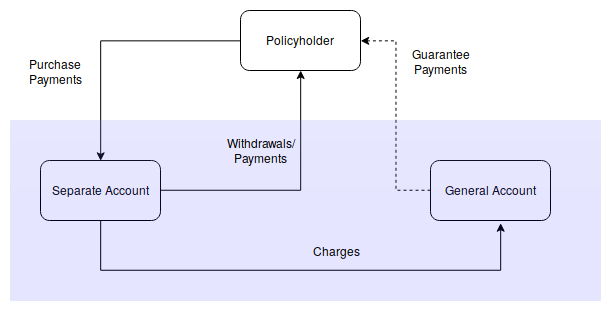
\includegraphics[width=\linewidth]{figure1.png}
   			\caption{VA fluxogram}
  		\end{subfigure}
  		\begin{subfigure}[b]{0.4\linewidth}
   			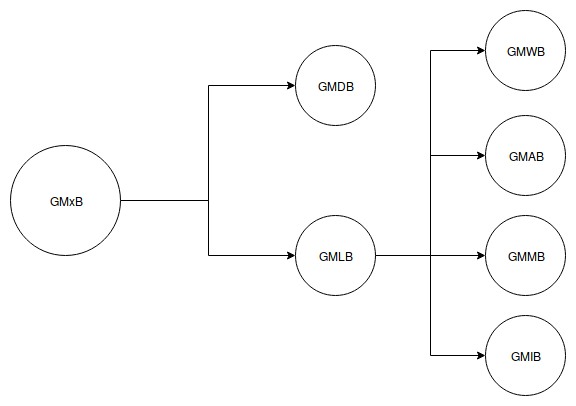
\includegraphics[width=\linewidth]{figure2.png}
    		\caption{Guarantees}
  		\end{subfigure}
  		\caption{Variable Annuity Description}
  		\label{fig:coffee}
		\end{figure}
	}
	\frame {
		\frametitle{Introduction}
		\setbeamertemplate{itemize items}[ball]		
		\begin{itemize}
			\setlength\itemsep{0,5em}
			\item Types of products:
			\begin{itemize}
				\item Guaranteed minimum death benefit (GMDB) 
				\item Guaranteed minimum withdrawal benefit (GMWB)
				\item Guaranteed minimum income benefit (GMIB)
				\item Guaranteed minimum maturity benefit (GMMB)
				\item Guaranteed minimum accumulation benefit (GMAB)
			\end{itemize}
			\end{itemize}
	}
	\frame {
		\frametitle{Introduction}
		\setbeamertemplate{itemize items}[ball]		
		\begin{itemize}
			\setlength\itemsep{0,5em}
			\item Using dynamic headging to mitigate the financial risks associated with VA guarantees, insurance companies first have to quantify the risks.
			\item This usually requires calculating the fair market values (FMV) of the guarantees for large portfolio of
VA contracts in a timely manner.
 			\item The value of the guarantees cannot be determined by closed-form formula.
 			\item Monte Carlo simulation can be used to value the VA protfolio, but it is extremly time-consuming
because every contract needs to be projected over many scenarios for a long time horizon.
			\end{itemize}
	}
	\frame {
		\frametitle{Introduction}
		\setbeamertemplate{itemize items}[ball]		
		\begin{itemize}
			\setlength\itemsep{0,5em}
			\item In order to deal with this problem, metamodeling approaches have been proposed to address the aforementioned computational problem.
			\item Using metamodeling approaches can reduce significantly the runtime of valuing a large portfolio of VA contracts for two main reasons:
			\begin{itemize}
				\item Building a metamodel only requires using the Monte Carlo simulation model to value a small number of
representative VA contracts
				\item The metamodel is usually much simpler and faster than the Monte Carlo simulation model.
			\end{itemize}
			\end{itemize}
	}
	\frame {
		\frametitle{Introduction}
		\setbeamertemplate{itemize items}[ball]		
		\begin{figure}
 			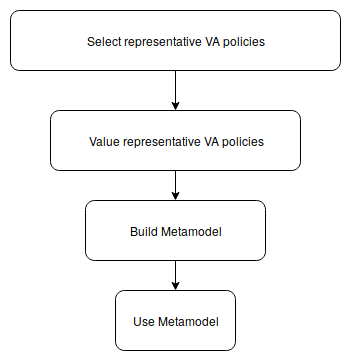
\includegraphics[width=0.6\linewidth]{figure3.png}
   			\caption{Metamodel fluxogram}
 		\end{figure}
	}
	\frame {
		\frametitle{Introduction}
		\setbeamertemplate{itemize items}[ball]		
		\begin{itemize}
			\setlength\itemsep{0,5em}
			\item In other words it consists in:
			\begin{itemize}
				\item Define a subset of representative VA contract.
				\item Compute the FMV for this represntative set using MC simulation.
				\item Fit a model based on the characteristics and FMV of the contracts
				\item Use the estimated model to predict the FMV of the remaining VA contracts.
			\end{itemize}
			\item The metamodels investigated in literature are sophisticated predictive models, which might cause difficulties in
terms of interpretation or calibration.
			\end{itemize}
	}
	\frame {
		\frametitle{Introduction}
		\setbeamertemplate{itemize items}[ball]		
		\begin{itemize}
			\setlength\itemsep{0,5em}
			\item The scope of this work is to investigate interaction terms in Generalized Linear
Model framework as a metamodel for valuing the complex financial guarantees associated with VA contracts. 
			\item We choose statiscally significant interaction terms to the model, evaluate performance as predictive model, and interpret the resulting effect of the addition of interaction terms. 
			\item We propose others metamodels: Box Cox regression and Neural Network regression. After describe these methods we will compare both e suggest the best of them to evaluate a VA portfolio.
		\end{itemize}
	}
	
	\frame {
		\frametitle{Review}
		\setbeamertemplate{itemize items}[ball]		
		\begin{itemize}
			\setlength\itemsep{0,5em}
			\item There are many publications on metamodeling approaches and recently these approaches have been proposed to speed up the valuation of large VA portfolios and produce accurate results.
			\item Some of the metamodels proposed and examined can be listed below:
			\begin{itemize}
				\item Ordinary Kriging
				\item Universal Kriging
				\item GB2 regression model
				\item Rank-order Kriging (quantile Kriging)
				\item Linear models with interactions
				\item Tree-based models 
			\end{itemize}
			
		\end{itemize}
	}
	
	\frame {
		\frametitle{Review}
		\setbeamertemplate{itemize items}[ball]		
		\begin{itemize}
			\setlength\itemsep{0,5em}
			\item In Gan (2018) author investigated the effect of including interactions in linear regression models for the valuation of those large VA portfolios. Since there were many features of VA contract, there were a large number of possible interactions between the features. So he selected the important interactions using overlaped group-lasso that could produce hierarchical interaction models. The numeric results obtained in Gan (2018) show that including interactions in linear regression
models can lead to significant improvements in prediction accuracy.
			\item In Gan and A.Valdez (2017), GB2 distribution was used to model the fair market values of VA guarantees, because it can captures the skewness shown in the empirical distribution of them. The GB2 distribution is a flexible statistical distribution that contains three shape parameters and one scale parameter.		
		\end{itemize}
	}
	
	\frame {
		\frametitle{Review}
		\setbeamertemplate{itemize items}[ball]		
		\begin{itemize}
			\setlength\itemsep{0,5em}
			\item The numerical results of that approach show that the four-stage optimization,described in that article, worked well and the result fitted in GB2 regression model performed as expected. Some comparison was made by the authors: (1) GB2 model
captures skewness better than Kriging model, (2) GB2 model outperforms the Kriging model in computational speed, (3)GB2 model produces comparably accurate predictions as teh Kriging model at portfolio level.
			\item An important step in the metamodeling process is the selection of representative policies. Gan and Valdez (2016) compared five different experimental design methods for the GB2 regression model:
			\begin{itemize}
			\item Random Sampling
			\item Low-discrepancy sequence
			\item Data clustering (Hierarchical k-means)
			\item Latin Hypercube sampling
			\item Conditional Latin Hypercube sampling
			\end{itemize}
		\end{itemize}
	}
	
	\frame {
		\frametitle{Review}
		\setbeamertemplate{itemize items}[ball]		
		\begin{itemize}
			\setlength\itemsep{0,5em}
			\item Hejazi and Jackson (2016), proposed a machine learning approach inside the metamodel. After a small set of representative VA contracts was selected and valued via Monte Carlos simulations, the values of these representatives contracts
were then used in a spatial interpolation method that found the value of the contracts in the input portfolio as a linear combination of the values of the representative contracts.		
			\item The traditional spatial interpolation methods as Kriging, IDW and RBF (Hejazi 2015) have a strong dependence with the distance function used in estimations. So authors proposed a neural network implementation of the spatial interpolation
techinique that learns an effective choice of that distance function. The results obtained by the authors show the superior accuracy of the neural network approach in estimation of the delta value for the input portfolio compared to the traditional
spatial interpolation techniques.
		\end{itemize}
	}
	\frame {
		\frametitle{Review}
		\setbeamertemplate{itemize items}[ball]		
		\begin{itemize}
			\setlength\itemsep{0,5em}
			\item Xu et al.(2018) propose a moment matching machine learning (MMML) approach to compute dollar deltas, VaRs and CVaRs for large portfolios. There are two main contributions that coulb be highlighted from this paper:
			\begin{itemize}
				\item First, they proposed a moment matching method to compute annual dollar deltas, VaRs, and CVaRs for a single VA contract. Due to these selected scenarios, the moment matching method can compute the annual dollar deltas, VaRs and CVaRs as accurately as the nested simulations, but only takes far less computational time as nested simulations requires.
				\item The second contribution is that they combine the moment matching method with some classical machine learning methods to manage the risk of a large VA portfolio.
			\end{itemize}			 
			\item Their MMML approach can easily handle huge portfolios (which cannot be handled via the nested simulation method due to cost).
		\end{itemize}
	}
	\frame {
		\frametitle{Review}
		\setbeamertemplate{itemize items}[ball]		
\begin{center}
\tiny
\begin{tabular}{lll}
  \hline
  Publication & Experimental Design & Metamodel \\
  \hline
  Gan (2013) & Clustering & Kriging \\
  \hline
  Gan and Lin (2015) & Clustering & Kriging \\
  \hline
  Gan (2015) & LHS & Kriging \\
  \hline
  Hejazi and Jackson (2016) & Uniform sampling & Neural network \\
  \hline
  Gan and Valdez (2016) & Clustering, LHS & GB2 regression \\
  \hline
  Gan and Valdez (2017) & Clustering & gamma regression \\
  \hline
  Gan and Lin (2017) & LHS, conditional LHS & Kriging \\
  \hline
  Hejazi et al. (2017) & Uniform sampling & Kriging, IDW, RBF\\
  \hline
  Gan and Huang (2017) & Clustering & Kriging \\
  \hline
  Xu et al (2018) & Random sampling & Neural Network, regression trees \\
  \hline
  Gan and Valdez (2018) & Clustering & GB2 regression \\
  \hline
  Quan, Gan and Valdez (2019) & Clustering & Regression trees \\ 
  \hline
\end{tabular}
\end{center}
	}
	
	\frame {
		\frametitle{Synthetic Datasets}
		\setbeamertemplate{itemize items}[ball]		
		\begin{itemize}
			\setlength\itemsep{0,5em}
			\item It is difficult for researchers to obtain real datasets from insurance companies to assess the performance of those metamodeling techniques.
			\item \textbf{Solution:} Synthetic Datasets (GAN and A.VALDEZ - 2017)
			\item Synthetic Datasets are large portfolios of VA contracts based on the properties of real portfolios of VA. 
			\item Properties typically observed on real portfolios of VA contracts:
			\begin{itemize}
				\item Different contracts may contain different types of guarantees.
				\item The contract holder has the option to allocate the money among multiple investment funds.
				\item Real variable annuity contracts are issued at different dates and have different times to maturity. 
			\end{itemize}
			
		\end{itemize}
	}
	
	\frame {
		\frametitle{Synthetic Dataset}
		\setbeamertemplate{itemize items}[ball]	
		\begin{itemize}
			\setlength\itemsep{0,5em}
			\item VA contracts in the synthetic portfolios:
		\end{itemize}
		\begin{center}
		\tiny
		\begin{tabular}{l l l}
		\hline
		Product & Description                 & Rider Fee  \\
		\hline
		DBRP    & GMDB with return of premium & 0.25\%     \\
		\hline
		DBRU    & GMDB with annual roll-up     & 0.35\%     \\
		\hline
		DBSU    & GMDB with annual ratchet     & 0.35\%     \\
		\hline
		ABRP    & GMAB with return of premium & 0.50\%     \\
		\hline
		ABRU    & GMAB with annual roll-up     & 0.60\%     \\
		\hline
		ABSU    & GMAB with annual ratchet     & 0.60\%     \\
		\hline
		IBRP    & GMIB with return of premium & 0.60\%     \\
		\hline
		IBRU    & GMIB with annual roll-up     & 0.70\%     \\
		\hline
		IBSU    & GMIB with annual ratchet     & 0.70\%     \\
		\hline
		MBRP    & GMMB with return of premium & 0.50\%     \\
		\hline
		MBRU    & GMMB with annual roll-up     & 0.60\%     \\
		\hline
		MBSU    & GMMB with annual ratchet     & 0.60\%     \\
		\hline
		WBRP    & GMWB with return of premium & 0.65\%     \\
		\hline
		WBRU    & GMWB with annual roll-up     & 0.75\%     \\
		\hline
		WBSU    & GMWB with annual ratchet     & 0.75\%     \\
		\hline
		DBAB    & GMDB + GMAB with annual ratchet & 0.75\%     \\
		\hline
		DBIB    & GMDB + GMIB wwith annual ratchet     & 0.85\%     \\
		\hline
		DBMB    & GMDB + GMMB with annual ratchet     & 0.75\%     \\
		\hline
		DBWB    & GMDB + GMWB with annual ratchet & 0.90\% \\
		\hline
		\end{tabular}
		\end{center}	
	
}
	\frame {
		\frametitle{Synthetic Dataset}
		\setbeamertemplate{itemize items}[ball]
		
		\begin{itemize}
			\setlength\itemsep{0,5em}
			\item Parameter values used to generate the synthetic portfolio.
		\end{itemize}
		\begin{center}
		\tiny
		\begin{tabular}{l l l}
		\hline
		Feature & Value \\
		\hline
		Policyholder birth date & [1/1/1950,1/1/1980] \\
		\hline
		Issue date & [1/1/2000,1/1/2014] \\
		\hline
		Valuation date & 1/6/2014 \\
		\hline
		Maturity & [15,30]years \\
		\hline
		Initial account value & [50000,500000] \\
		\hline
		Female percent & 40\% \\
		\hline
		Fund fee & 30, 50, 60, 80, 10, 38, 45, 55, 57, 46 bps for Funds 1 to 10 \\
		\hline
		M\&E fee & 200 bps \\
		\end{tabular}
		\end{center}	
	
}
	\frame {
		\frametitle{Synthetic Dataset}
		\setbeamertemplate{itemize items}[ball]		
		\begin{itemize}
			\setlength\itemsep{0,5em}
			\item 10,000 synthetic variable annuity policies were generated for each of the guarantee types.
			\item The Synthetic portfolio contains 190,000 policies.
			\item There are 45 fields in total, including 10 fund values, 10 fund numbers and 10 fund fees. 
			\begin{center}
			\tiny
			\begin{tabular}{l l l}
			\hline
			Field & Description \\
			\hline
			recordID & Unique identifier of the policy \\
			\hline
			survivorShip & Positive weighting number\\
			\hline
			gender & Gender of the policyholder \\
			\hline
			productType & Product type \\
			\hline
			issueDate & Issue Date \\
			\hline
			matDate & Maturity date\\
			\hline
			birthDate & Birth date of the policyholder \\
			\hline
			currentDate & Current date\\
			\hline
			baseFee & M\&E (Mortality \& Expense) fee \\
			\hline
			riderFee & Rider fee \\
			\hline
			rollUprate & Roll-up rate\\
			\hline
			rollUprate & Guaranteed benefit\\
			\hline
			rollUprate & GMWB balance\\
			\hline
			wbWithdrawalRate & Guaranteed withdrawal rate\\
			\hline
			withdrawal & Withdrawal so far\\
			\hline
			FundValuei & Fund value of the ith investment fund\\
			\hline
			FundNumi & Fund number of the ith investment fund\\
			\hline
			FundFeei & Fund management fee of the ith investment fund\\
			\end{tabular}
			\end{center}
			
			\end{itemize}		
		}
\frame {
		\frametitle{Synthetic Dataset}
		\setbeamertemplate{itemize items}[ball]		
		\begin{itemize}
			\setlength\itemsep{0,5em}
			\item Monte Carlo simulation engine to calculate the fair market values (FMV), partial dollar deltas and partial dollar rhos of the guarantees for the synthetic portfolio.
			\item The total fair market value is positive, because the guarantee benefit payoff is more than the risk.
			\item Since the VA contracts are usually long-terms contracts, the guarantees are more sensitive to long-term interest rates than to short-term interest rates.
			\item The total amount of those variables are described above: 
			\begin{center}
			\tiny
			\begin{tabular}{l l l l}
			\hline
			Quantity Name & Value & Quantity Name & Value  \\
			\hline
			FMV & 18,572,095,089 & Rho2y & 167,704 \\
			\hline
			Delta1 & -4,230,781,199 & Rho3y & 85,967 \\
			\hline
			Delta2 & -2,602,768,996 & Rho4y & 2,856 \\
			\hline
			Delta3 & -2,854,233,170 & Rho5y & -96,438 \\
			\hline
			Delta4 & -2,203,726,514 & Rho7y & 546,045 \\
			\hline
			Delta5 & -2,341,793,581 & Rho10y & 1,407,669 \\
			\hline
			Rho1y & 40,479 & Rho30y & 62,136,376 \\
			\end{tabular}
			\end{center}
			
			\end{itemize}		
		}

\end{document}
